\documentclass[12pt, oneside]{article}   	% use "amsart" instead of "article" for AMSLaTeX format
\usepackage{geometry}                		% See geometry.pdf to learn the layout options. There are lots.
\geometry{letterpaper}                   		% ... or a4paper or a5paper or ... 
%\geometry{landscape}                		% Activate for for rotated page geometry
%\usepackage[parfill]{parskip}    		% Activate to begin paragraphs with an empty line rather than an indent
\usepackage{graphicx}				% Use pdf, png, jpg, or eps� with pdflatex; use eps in DVI mode
								% TeX will automatically convert eps --> pdf in pdflatex		
\usepackage{amssymb}
\usepackage{amsmath}
\usepackage{parskip}
\usepackage{color}

\title{Permutations and Combinations}
%\author{The Author}
%\section{}
% \subsection*{R code}
\date{}							% Activate to display a given date or no date

\graphicspath{{/Users/telliott_admin/Dropbox/Tex/png/}}

% \begin{center} 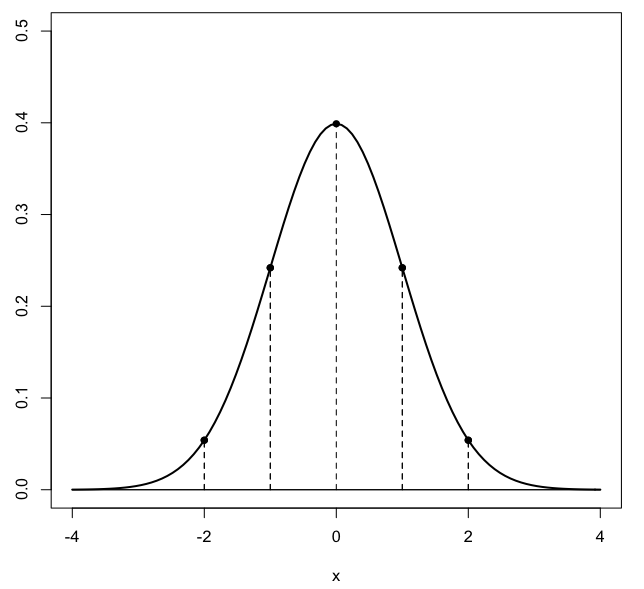
\includegraphics [scale=0.4] {gauss3.png} \end{center}
% \begin{bmatrix} a  &  b \\ c  &  d \end{bmatrix}
% \bigg |_

\begin{document}
\maketitle
%\noindent

Most people have heard an explanation of permutations somewhere in a math class.  Suppose we consider just the two letters $a$ and $b$.  These can be arranged in two orders, or permutations.  Either $a$ is first and $b$ second, or the reverse:

\[ ab \]
\[ ba \]

Either I eat pizza and then I eat ice cream, or I eat ice cream first and then pizza.

Now, how about $abx$?

One way to reason about this is to say that in starting with a sequence of length two like $ab$, there are three possible places to add a new letter---in front of or behind $ab$, or between the two characters.  So starting with $ab$ we would have

\[ xab \ \ axb \ \ abx \]

and starting with $ba$ we would have

\[ xba \ \ bxa \ \ bax \]

so that's a total of $3 \times 2 = 6$ possibilities.

Another way is to imagine a row of three boxes, where each box will hold a particular letter.  We pick one of the three letters for the first position (the first box), one of the two remaining for the second position, and for the third, we have no choice.

In general, for $n$ objects, there are $n \times n-1 \times \cdots \times 1 = n!$ possible orders.

I have 5 Bob Marley CDs.

There are $5! = 5 \times 4 \times 3 \times 2 \times 1 = 120$ orders in which I could play my five CDs tonight.  I want to hear them all, but I don't want to hear any particular CD more than once.  Here are two of the 120 possible orderings.

\begin{center} 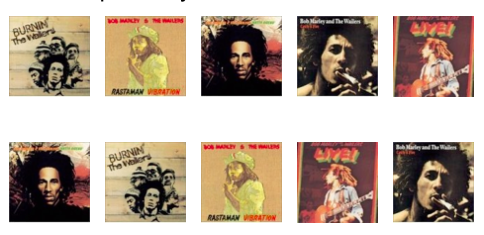
\includegraphics [scale=0.4] {bob.png} \end{center}

Now, suppose we consider the problem of picking not all $n$ objects in order, but instead a subset of $k$ objects from that total $n$.  For example, let's pick two CDs from the 5 above.  We could pick \emph{Burning} and the Live album, or another group of 2 like \emph{Catch A Fire} and \emph{Natty Dread}.

It's easy to see that the number of possibilities in this problem is $5 \times 4$, \emph{as long as the order is important}.

But suppose we don't want to do that.  Instead, we want to say that (\emph{Catch A Fire}, \emph{Natty Dread}) is the same as (\emph{Natty Dread}, \emph{Catch A Fire}).  We like Bob Marley, but listening to the same album twice in one night is just too much.  These are called "combinations."

Let's look at it with letters.  Suppose we have $n=5$ letters $abcde$ and we want to pick just $k=2$.  We can pick any of 5 for the first, then any one of the four remaining so there are $5 \times 4 = 20$ possibilities, when considering the ordered pairs.

\[ ab \ \ ac \ \ ad \ \ ae \]
\[ ba \ \ bc \ \ bd \ \ be \]
\[ ca \ \ cb \ \ cd \ \ ce \]
\[ da \ \ db \ \ dc \ \ de \]
\[ ea \ \ eb \ \ ec \ \ ed \]

How many duplicates are there?  For every pair like $x,y$, the reverse ordering $y,x$ is also present.

For any ordering of $k$ items, there are $k!$ permutations (all the permutations of different orderings but containing exactly the same elements).  We will have to correct our count by dividing by $k!$.  

In general, if we have $n$ total items and choose $k$ of them, we have $k$ terms multiplied together starting with $n \times (n-1) \times  \cdots$:

\[ n \times (n-1) \]
\[ 5 \times 4 =  20 \]

To get the number of combinations we divide by $k!$, which here equals $2$, giving us $10$ combinations of $k=2$ objects from a total collection of $n=5$ objects.

A second issue is how we compute the number of orders.  To get $k$ terms from $n$ total objects, we do

\[ n \times (n-1) \cdots \times (n-k+1) \]

It's a bit tricky, but I hope it is clear that for $k=2$ the last term is $n-2+1 = n-1$ and for $k=3$ the last term is $n-3+1 = n-2$ and so on.


In summary, to count the combinations with $k$ items picked from a set of $n$ total items

\[ C = \frac{1}{k!} \ \ n \times (n-1) \cdots \times (n-k+1) \]

That's basically it, but we can simplify by considering one last thing.

\[ n! = n \times (n-1) \cdots \times (n-k+1) \times (n-k) \cdots \times 2 \times 1 \]

so

\[ \frac{n! }{(n-k)!} = \frac{n \times (n-1) \cdots \times (n-k+1)}{1} \times \frac{(n-k) \cdots \times 2 \times 1}{(n-k) \cdots \times 2 \times 1 } \]
\[ = n \times (n-1) \cdots \times (n-k+1) \]

Therefore, we can rewrite the expression for $C$ above

\[ C = \frac{1}{k!} \ \ n \times (n-1) \cdots \times (n-k+1) \]
\[ = \frac{n!}{k! \ (n-k)!} \]

This is commonly written 

\[ C = {n \choose k} = \frac{n!}{k! \ (n-k)!} \]

Notice the symmetry

\[ {n \choose k} = \frac{n!}{k! \ (n-k)!} = {n \choose n-k} \]

If I pick two cards from a deck of 52, that is the same problem as picking 50 out of 52, because all I really need to do for the latter  is to pick the two to leave behind.

\end{document}  